%%% fs-state-experiments - Experiments

\label {fs-experiments-seciton}

The series of experiments were performed in order to analyze the overall performance of the proposed approach. For experiments, we use an open-source implementation of the drifting state model called~\FlameStream\ . \FlameStream\ is a distributed stream processing engine implemented in Java using Akka framework. \FlameStream\ can be deployed on a hardware cluster of computational units that we call nodes. We assume that each node is connected through a network with all other nodes.

\begin{figure*}[htbp]
  \centering
  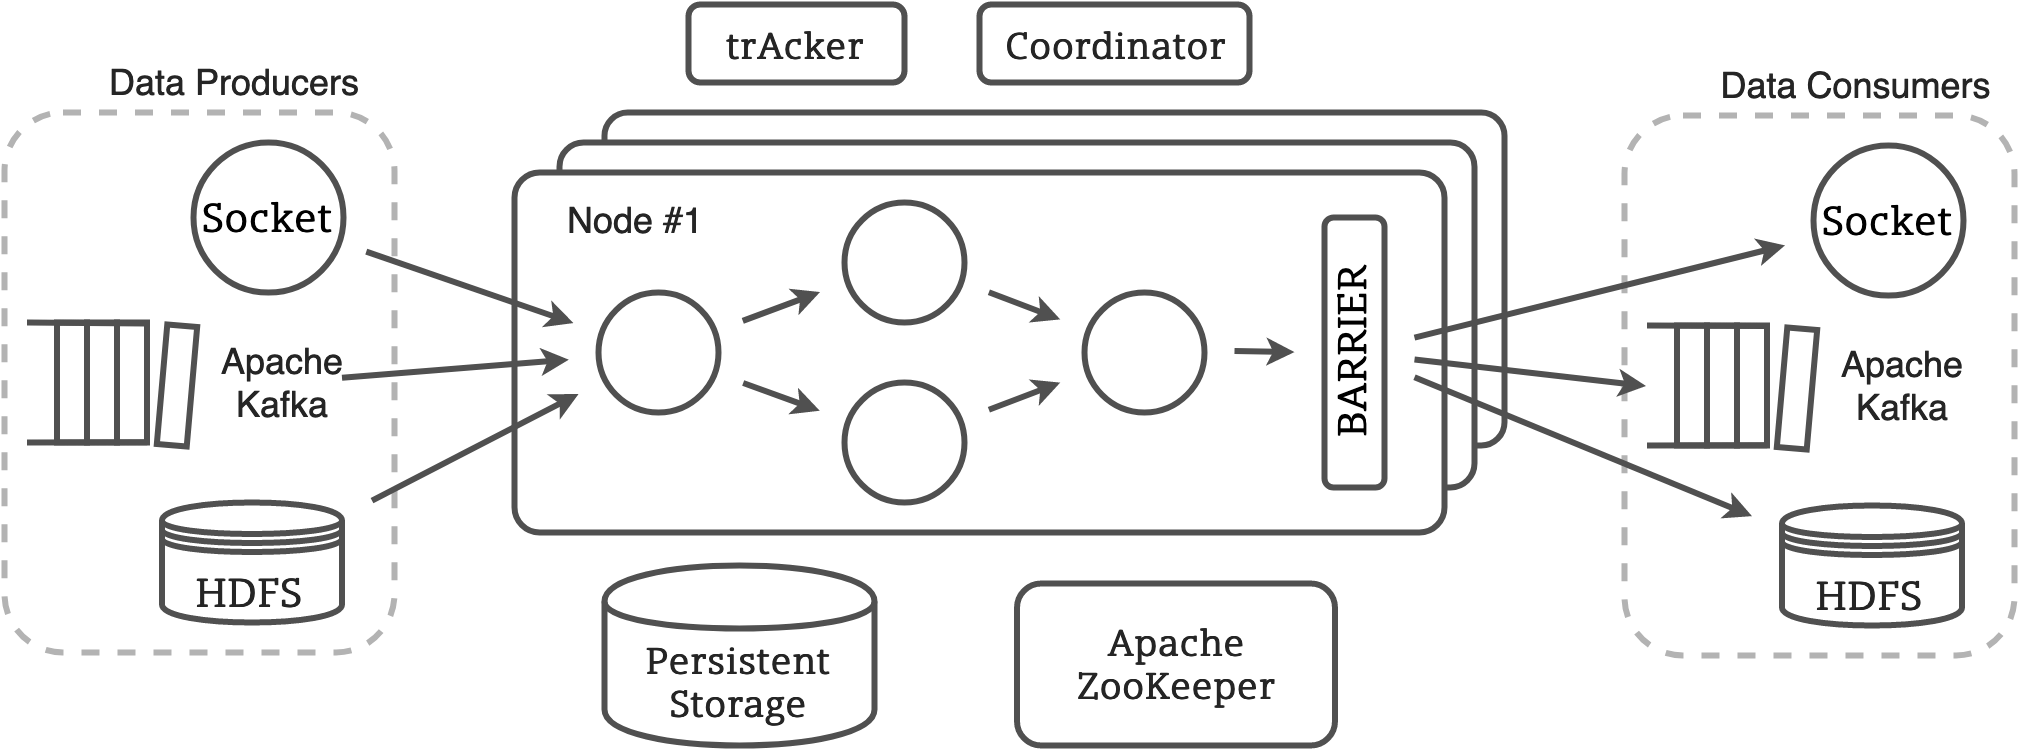
\includegraphics[scale=0.78]{pics/arch}
  \caption{The overview of \FlameStream\ architecture}
  \label {arch}
\end{figure*}

An overview of the \FlameStream\ architecture is shown in Figure~\ref{arch}. The roles of the barrier, \Acker\ , coordinator, cluster state manager, data producers, and data consumers are detailed in the previous sections. The other components are:

{\bf Node} runs a process called {\it worker}. Worker executes user-defined operations. The computational load is balanced through the distribution of data items among workers. A worker for a data item is determined by the value of a hash function of item payload. Such hash functions can be defined by a user before each logical operation. Each worker can be responsible for one or many ranges of values of hash functions called {\it hash units}. The number of hash-units per worker is a user-defined parameter, and it must be set before the start of computations. 

{\bf Execution graph} is an Akka-based representation of a user-defined logical graph. Execution graph is run by each worker. A data item can be sent to another worker before each operation due to balancing technique and the distribution of hash units. The communication within a node is done via messaging or direct function calls depending on runtime heuristics. A delivery that crosses node boundaries is performed by means of TCP.

{\bf Persistent storage} is needed for reliable storing of state snapshot. In case of failures, the state snapshot is recovered from persistent storage. It can be a distributed file system or database (e.g., HDFS, S3, MongoDB, GFS, HBase, etc.).

\subsection{Setup}
We apply building an inverted index as a stream processing task for the evaluation. Building inverted index is implemented as a MapReduce transformation in a streaming manner. The scheme is shown in Figure~\ref{index}: 

\begin{itemize}
    \item Map phase includes conversion of input documents into the key-value pairs {\it (word; word positions within the page)}
    \item Reduce phase consists of combining word positions for the corresponding word into the single index structure 
\end{itemize}

Reduce phase outputs the change records of the inverted index structure, to make this algorithm suitable for stream processing systems. It implies that each input page triggers the output of the corresponding change records of the full index. In \FlameStream\ this algorithm is implemented as the typical conversion of MapReduce transformation, which is shown in~\cite{we2018seim}.

\begin{figure}[htbp]
  \centering
  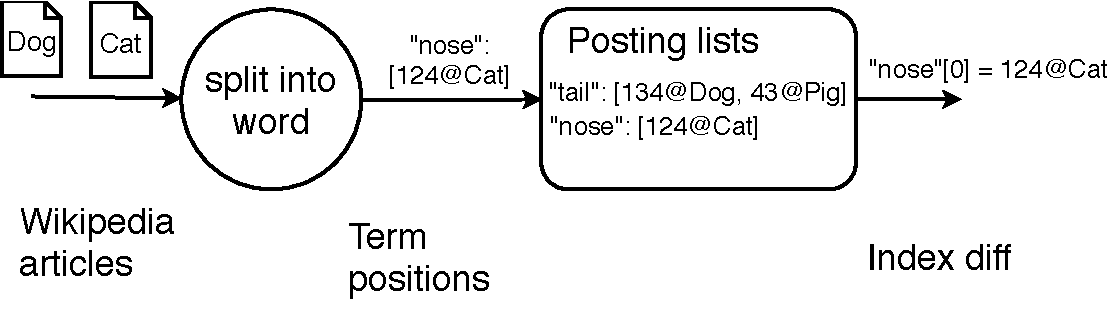
\includegraphics[width=0.50\textwidth]{pics/index}
  \caption{The inverted index pipeline}
  \label {index}
\end{figure}

We chose the task of building an inverted index because it satisfies the following properties:

\begin{itemize}
    \item Operation that generates change records is non-commutative
    \item The computational pipeline of the task contains network shuffle that can violate the ordering constraints
    \item Consistency guarantees are strongly required because the inconsistent index does not make sense for many applications
    \item The workload is unbalanced due to Zipf's law
\end{itemize}

Notably, building an inverted index in a streaming manner can be the halfway task between the generation of documents and consuming index updates by search infrastructure. In the real world, this scenario can be found in freshness-aware systems, e.g., news processing engines.

By the notion of {\it latency} we assume the time between two events: 

\begin{enumerate}
    \item Input page is taken into the stream
    \item All the change records for the page leave the stream
\end{enumerate}

Our experiments were performed on the cluster of 10 Amazon EC2 micro instances with 1GB RAM and 1 core CPU. We used Wikipedia articles as a dataset. Documents per second input rate is 50. RocksDB~\cite{rocksdb} is used as a storage for the state. The role of data producer and data consumer is played by a custom server application that sends and receives data through socket and measures the latency.

\subsection{Overhead and recovery}
The performance of the proposed deterministic model within the same stream processing task is deeply analyzed in~\cite{we2018seim}. In this paper, we aim to evaluate the overhead on providing consistency guarantees and the time needed for the full recovery.

Figures~\ref{comparison50}, ~\ref{comparison500}, and ~\ref{comparison1000} shows the latencies of \FlameStream\ within distinct times between checkpoints. As expected, the overhead on exactly once enforcement is low (less than 10 ms), and it does not depend on the time between checkpoints. Slight overhead can be explained by the fact that asynchronous state snapshotting is executed on single-core nodes. The time between checkpoints does not influence latency because output elements delivery and state snapshotting mechanisms are independent in our model.

System's behavior in case of failures and recoveries is demonstrated in Figure~\ref{recovery}. It is shown that the system can perform recovery processes in an adequate time. Existing latency spikes are caused by the replay process, JVM restart, etc.

\begin{figure}[htbp]
  \centering
  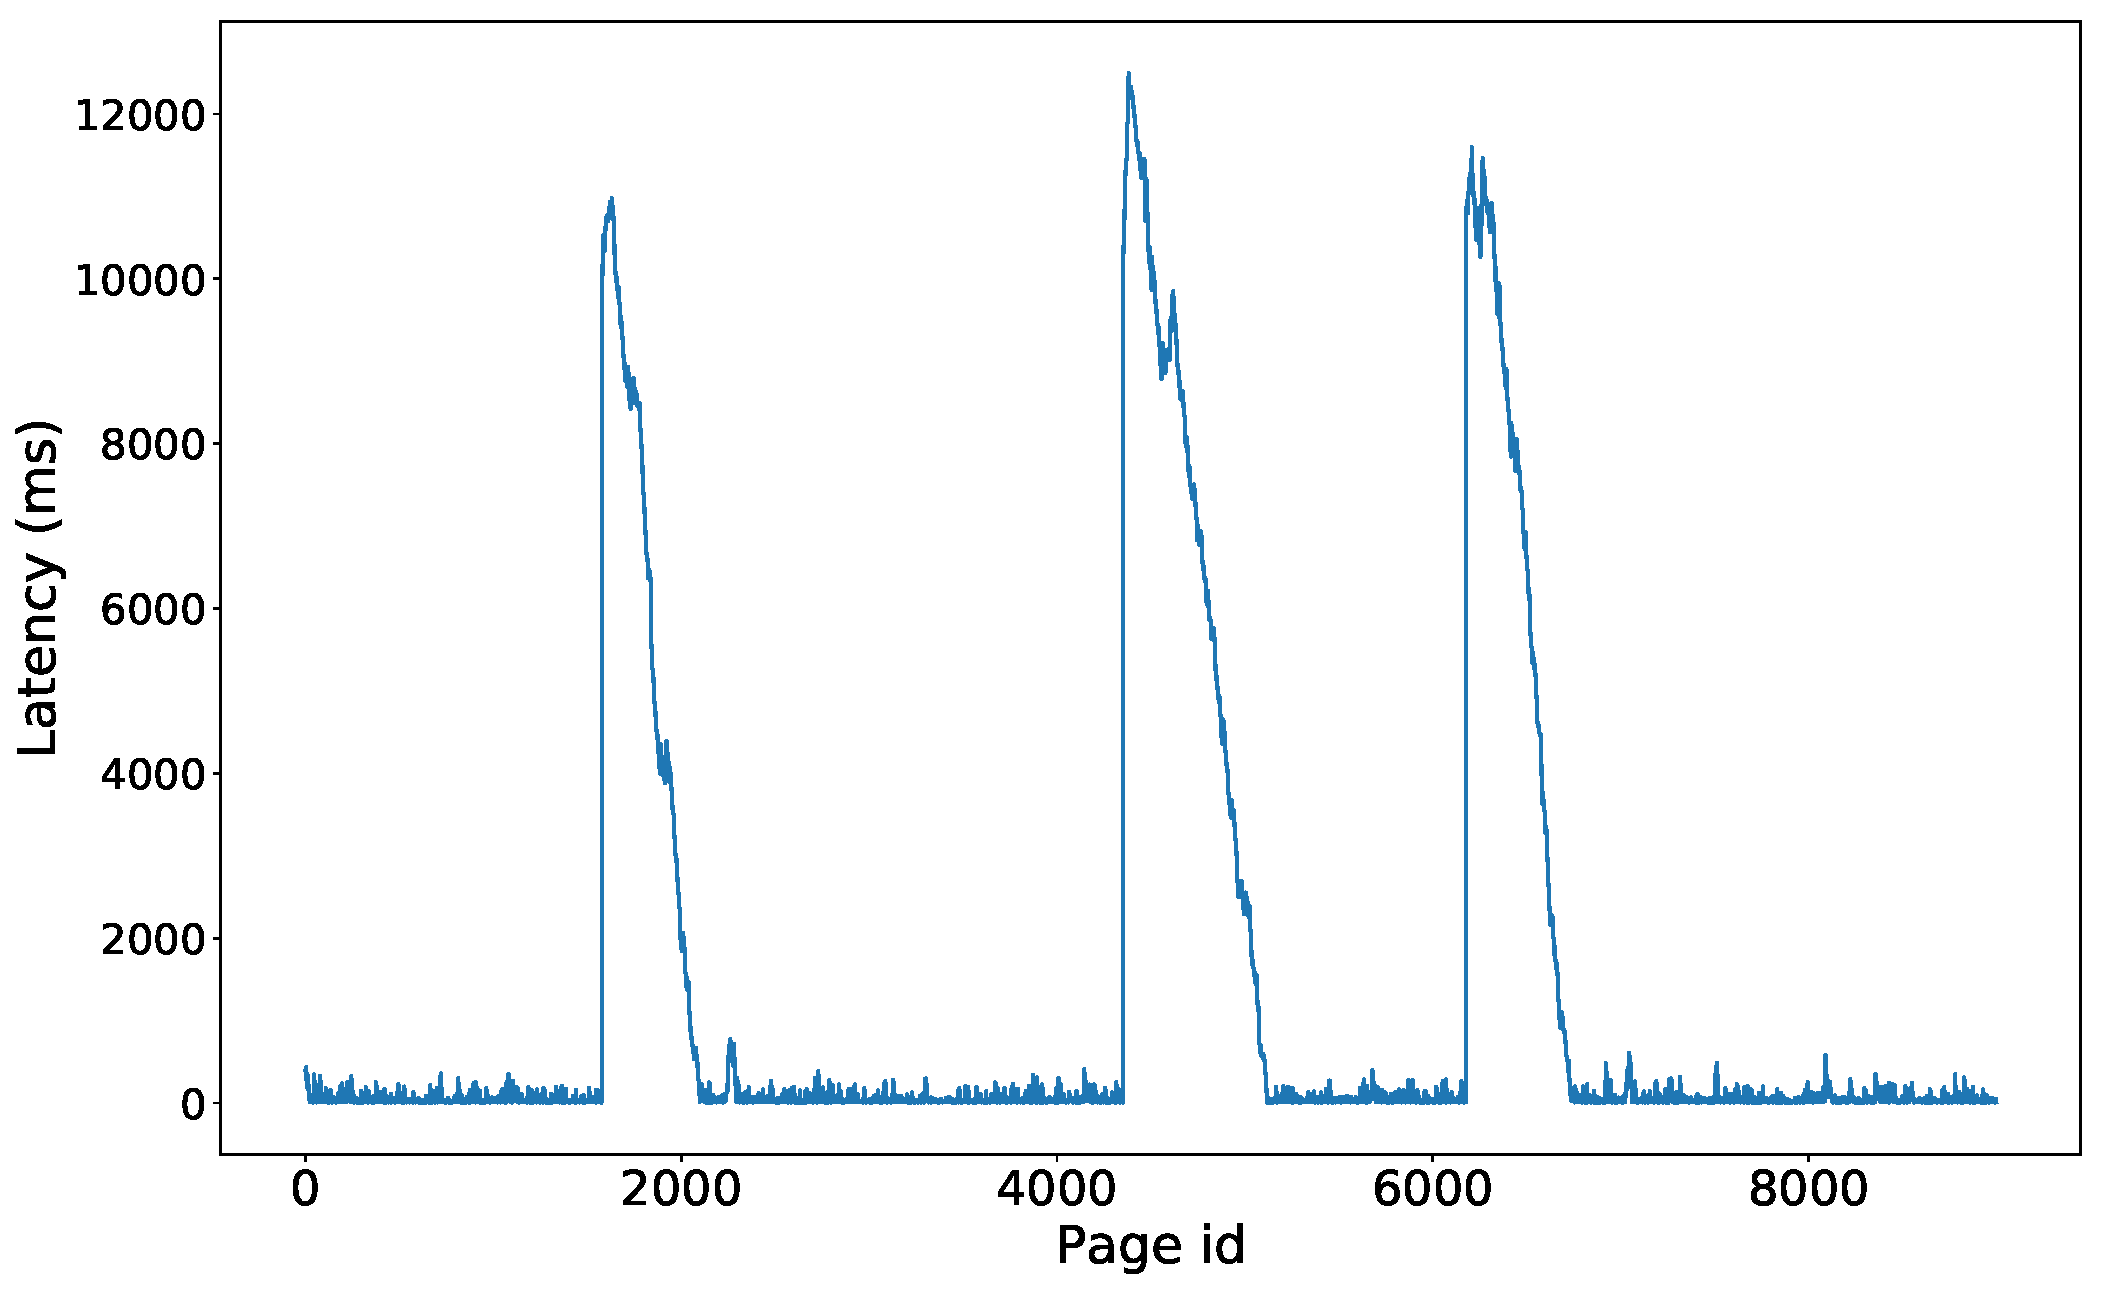
\includegraphics[width=0.48\textwidth]{pics/blink}
  \caption{The latencies of \FlameStream\ during three failures and recoveries}
  \label {recovery}
\end{figure}

\subsection{Comparison with an industrial system}
One of the most important goals of the experiments is the performance comparison with an industrial solution regarding latency. Apache Flink has been chosen for evaluation because it is a state-of-the-art stream processing system that provides similar functionality and achieves low latency in the real-world scenarios~\cite{S7530084}. 

For Apache Flink, the algorithm for building the inverted index is adopted by the usage of {\it FlatMapFunction} for map step and stateful {\it RichMapFunction} for reduce step and for producing the change records. The network buffer timeout is set to 0 to minimize latency. Custom {\it TwoPhaseCommitSinkFunction} that buffers output items in memory until a transaction is committed is used for experiments that require exactly-once semantics. 

{\it FsStateBackend} with the local file system is used for storing the state, because {\it RocksDBStateBackend} requires saving state to RocksDB on each update that leads to additional overhead. {\it FsStateBackend} stores state on the disk only on checkpoints and do not provide an additional overhead against RocksDB storage in \FlameStream, so it is fairer to use it rather than {\it RocksDBStateBackend} for comparison purposes.

In this paper, we compare $50^{th}$, $75^{th}$, $95^{th}$, and $99^{th}$ percentile of distributions, which clearly represent the performance from the perspective of the users' experience.

\begin{figure}[htbp]
  \centering
  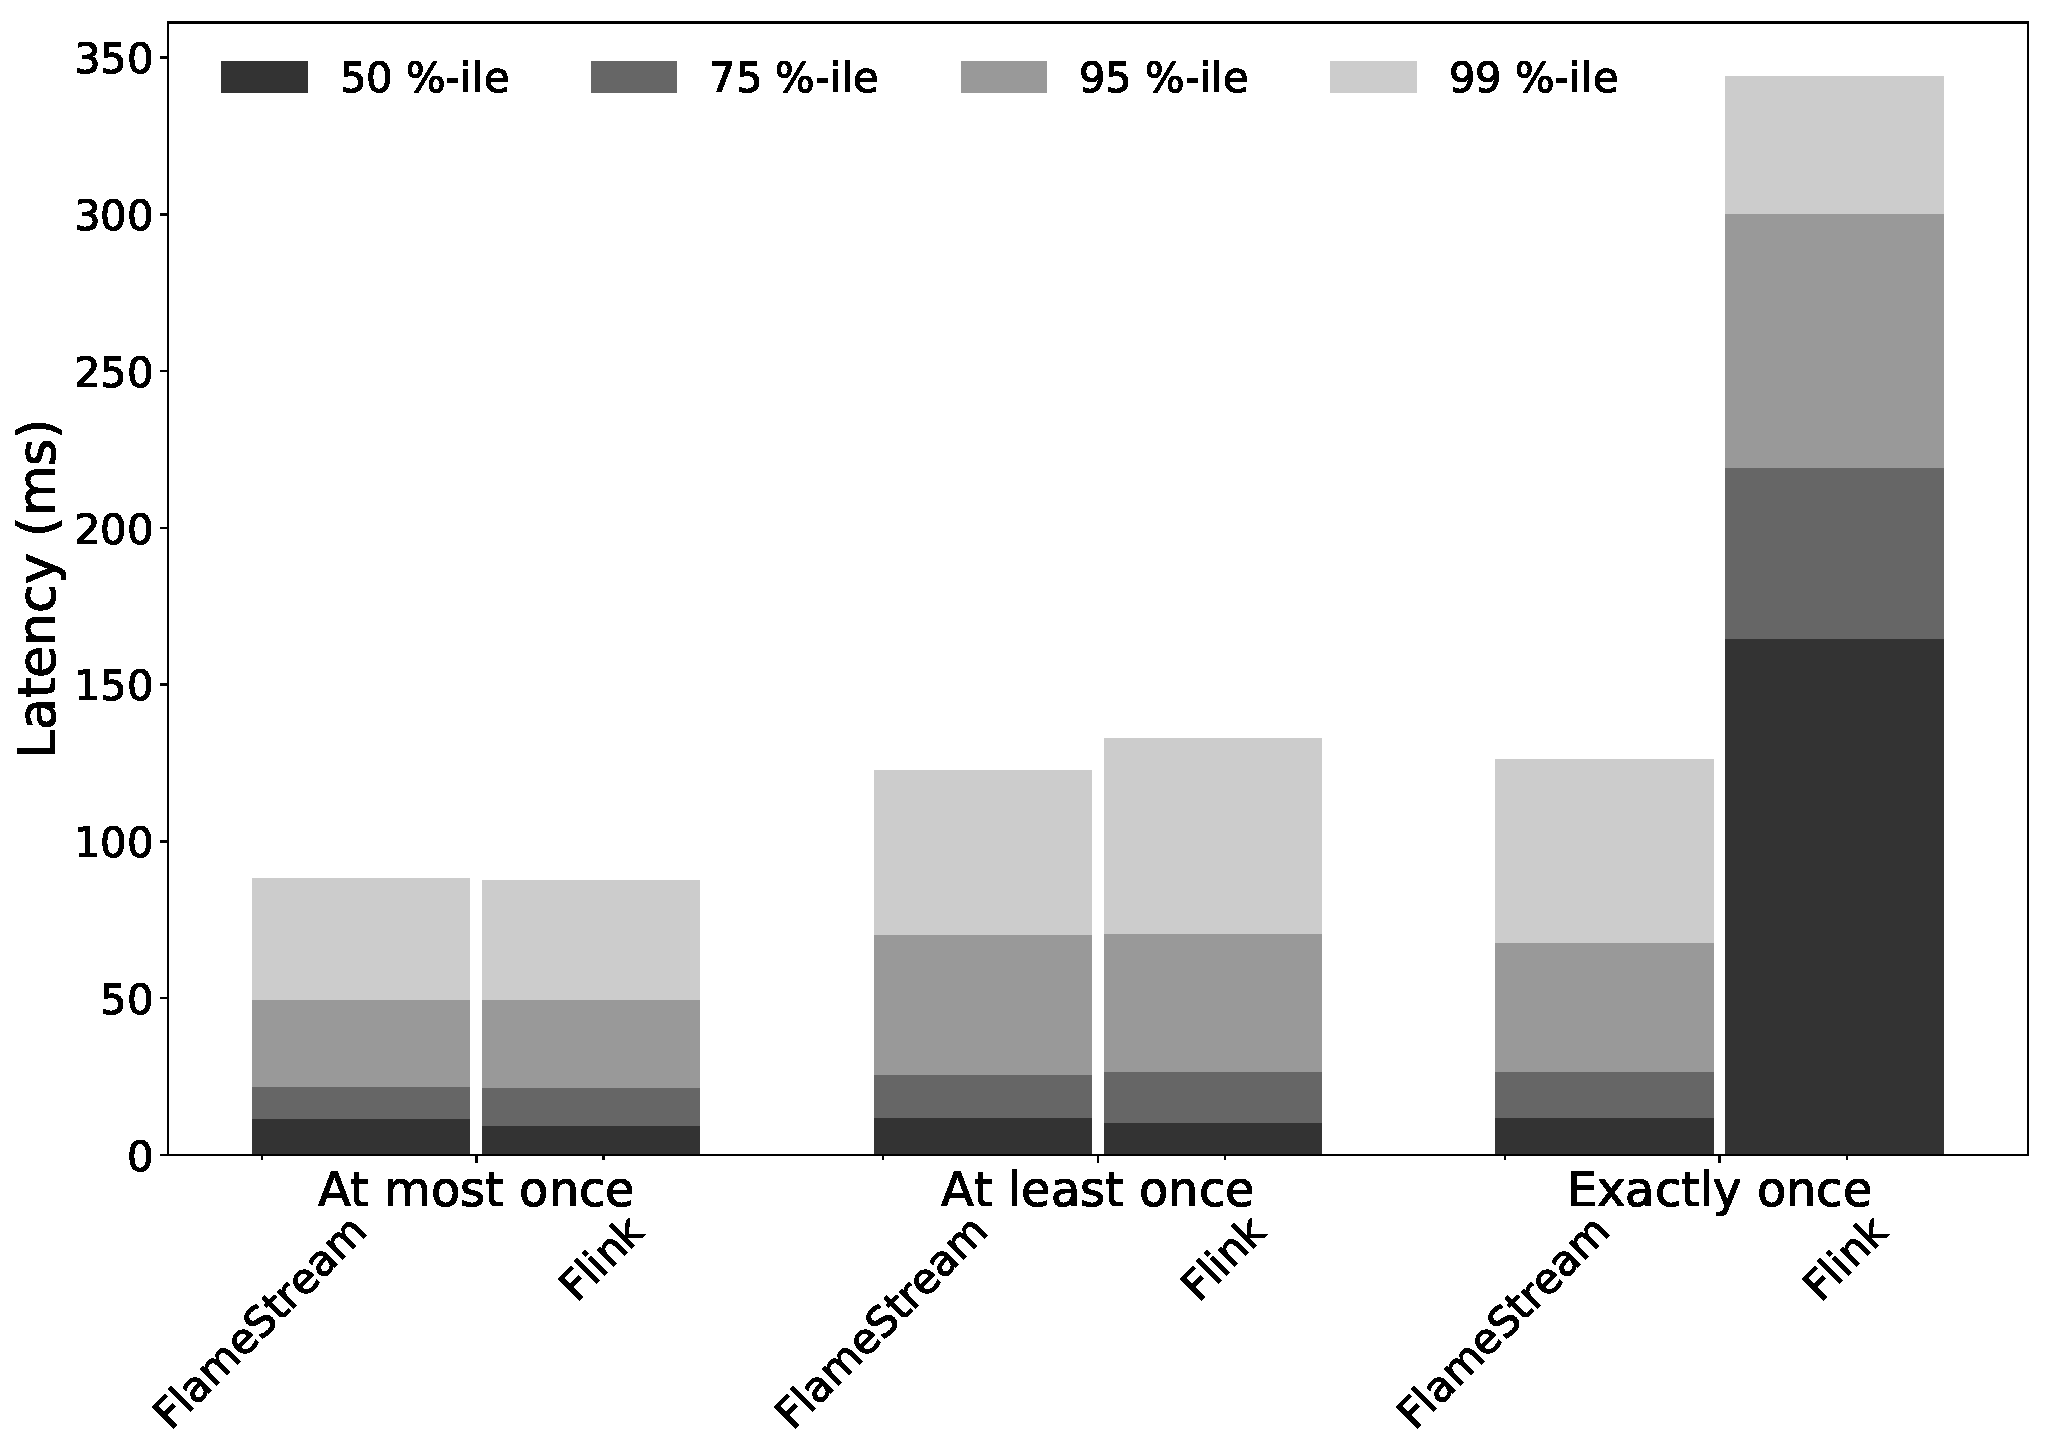
\includegraphics[width=.5\textwidth]{pics/comparison50}
  \caption{The comparison in latencies between \FlameStream\ and Flink with 50 ms delay between checkpoints}
  \label {comparison50}
\end{figure}

Figures~\ref{comparison50}, ~\ref{comparison500}, and ~\ref{comparison1000} demonstrates the comparison of latencies between \FlameStream\ and Flink within distinct times between checkpoints, and different guarantees on data. Without guarantees, the latencies of \FlameStream\ and Flink do not significantly differ. However, for exactly once, Flink's latency is dramatically higher, and it directly depends on the time between checkpoints. Nevertheless, such behavior is expected, because Flink needs to take state snapshot and release output items within a single transaction to ensure that all states of non-commutative operations are persistently saved. There are no hints implemented in Flink which could mark an operation as commutative, hence it waits until states of all operations are stored before output delivery. On the other hand, the property of determinism allows \FlameStream\ to not synchronize state snapshotting and output delivery. This fact makes it possible to achieve exactly once with low overhead.

\begin{figure}[htbp]
  \centering
  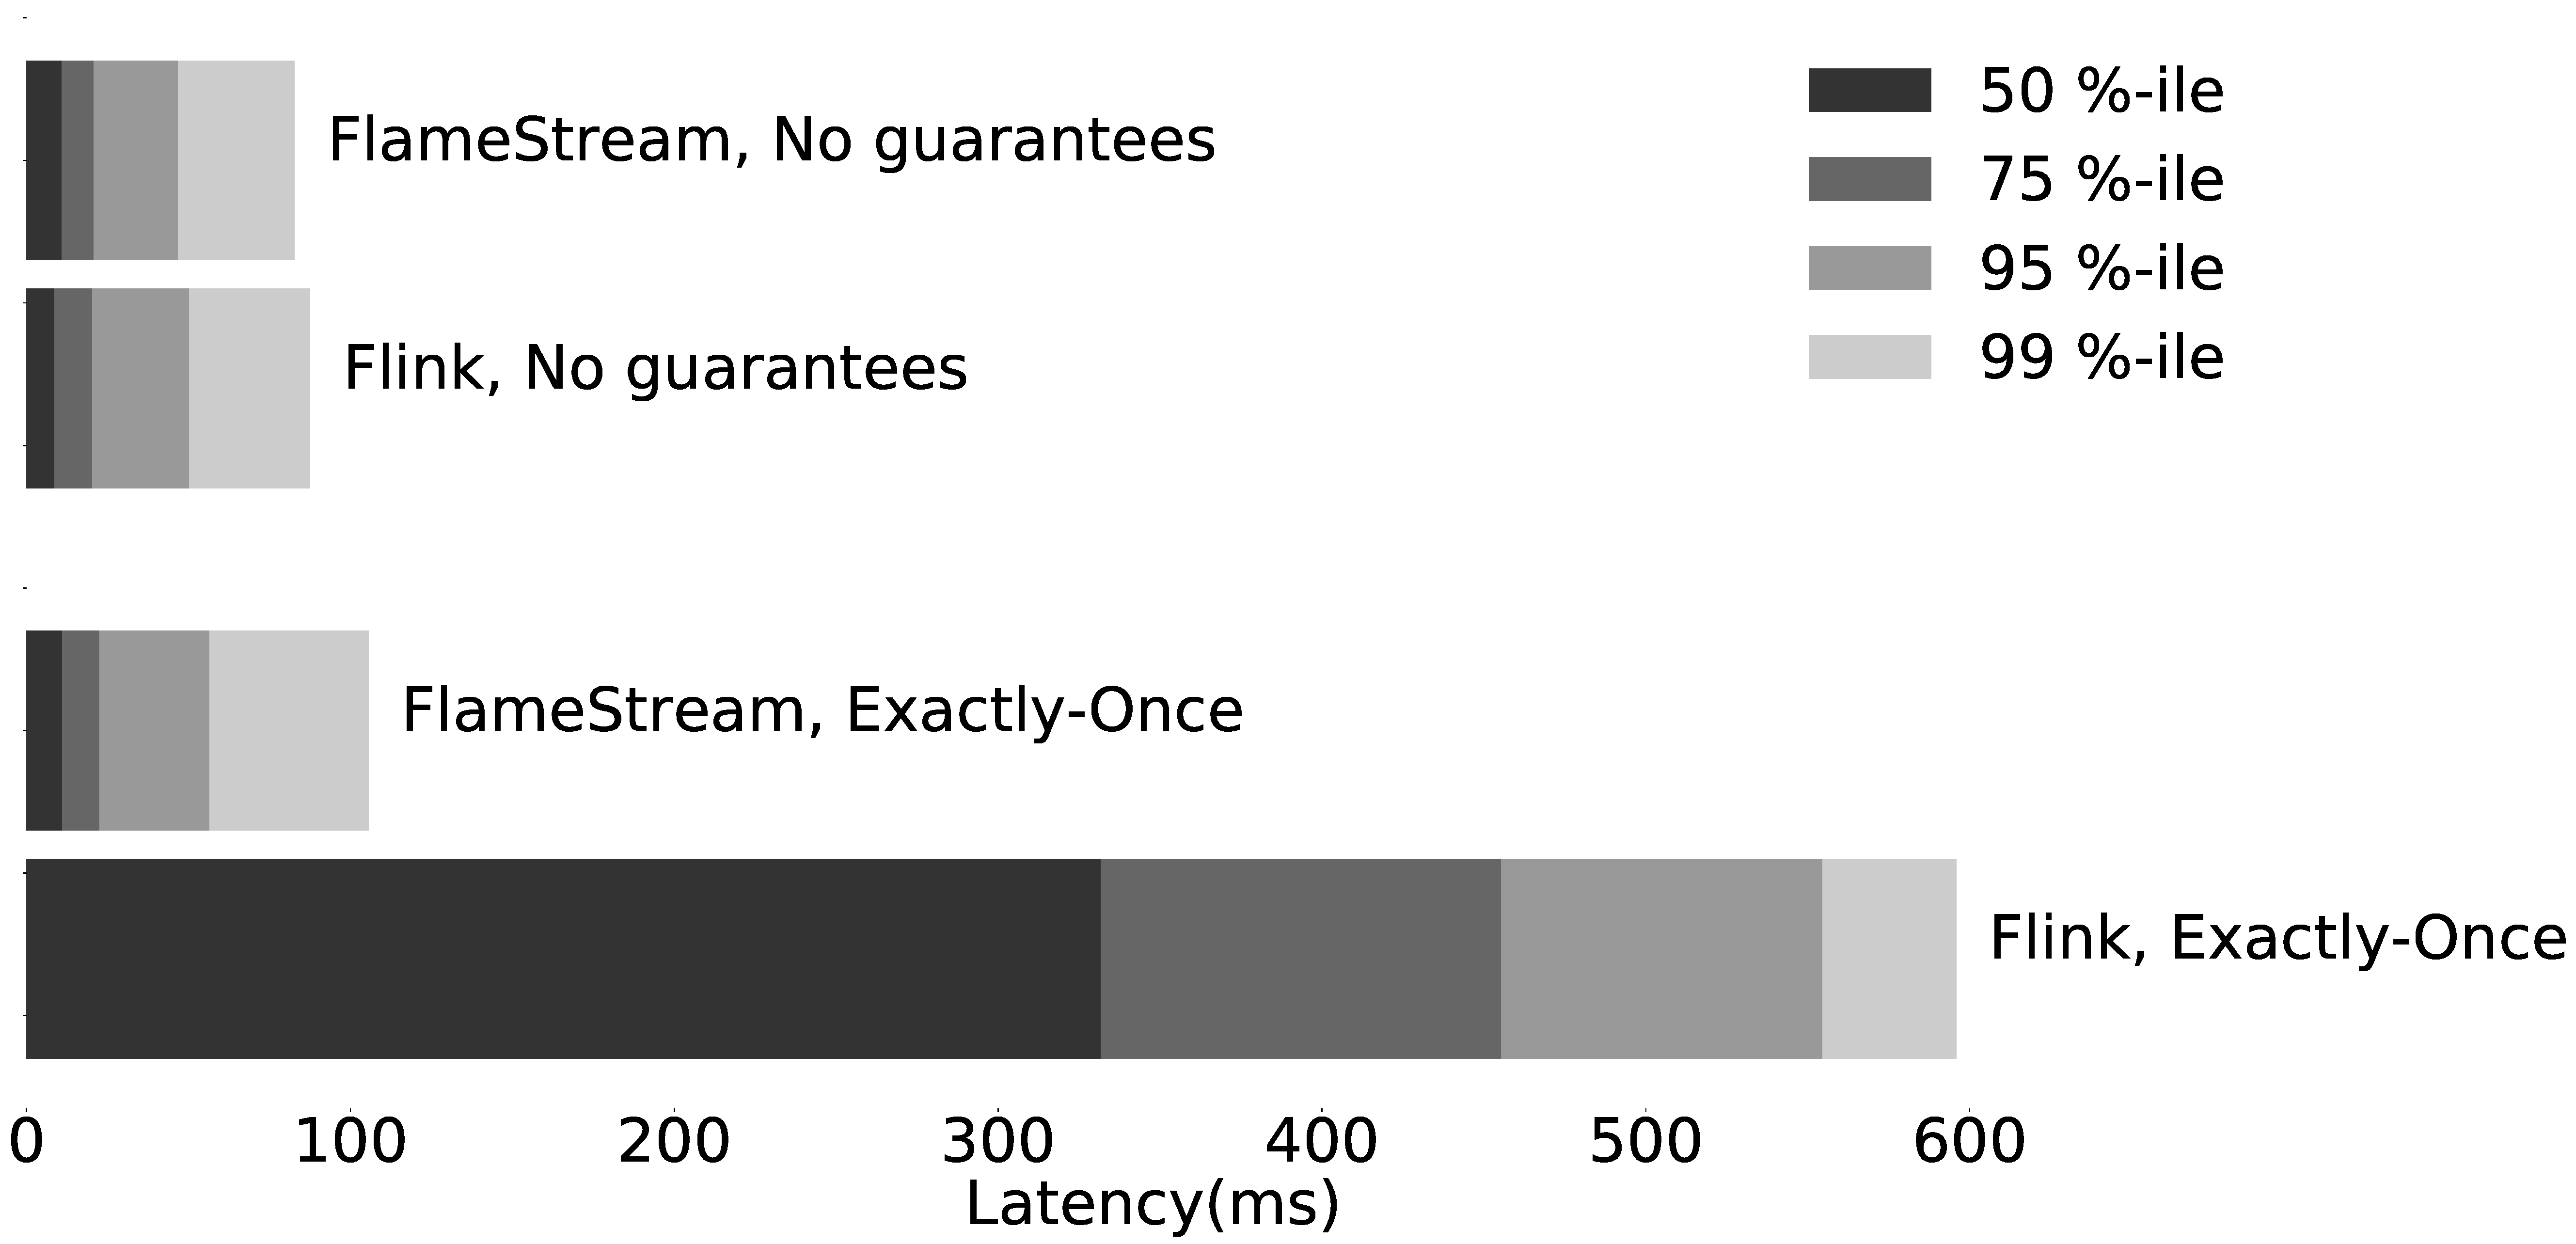
\includegraphics[width=.5\textwidth]{pics/comparison500}
  \caption{The comparison in latencies between \FlameStream\ and Flink with 500 ms delay between checkpoints}
  \label {comparison500}
\end{figure}

\begin{figure}[htbp]
  \centering
  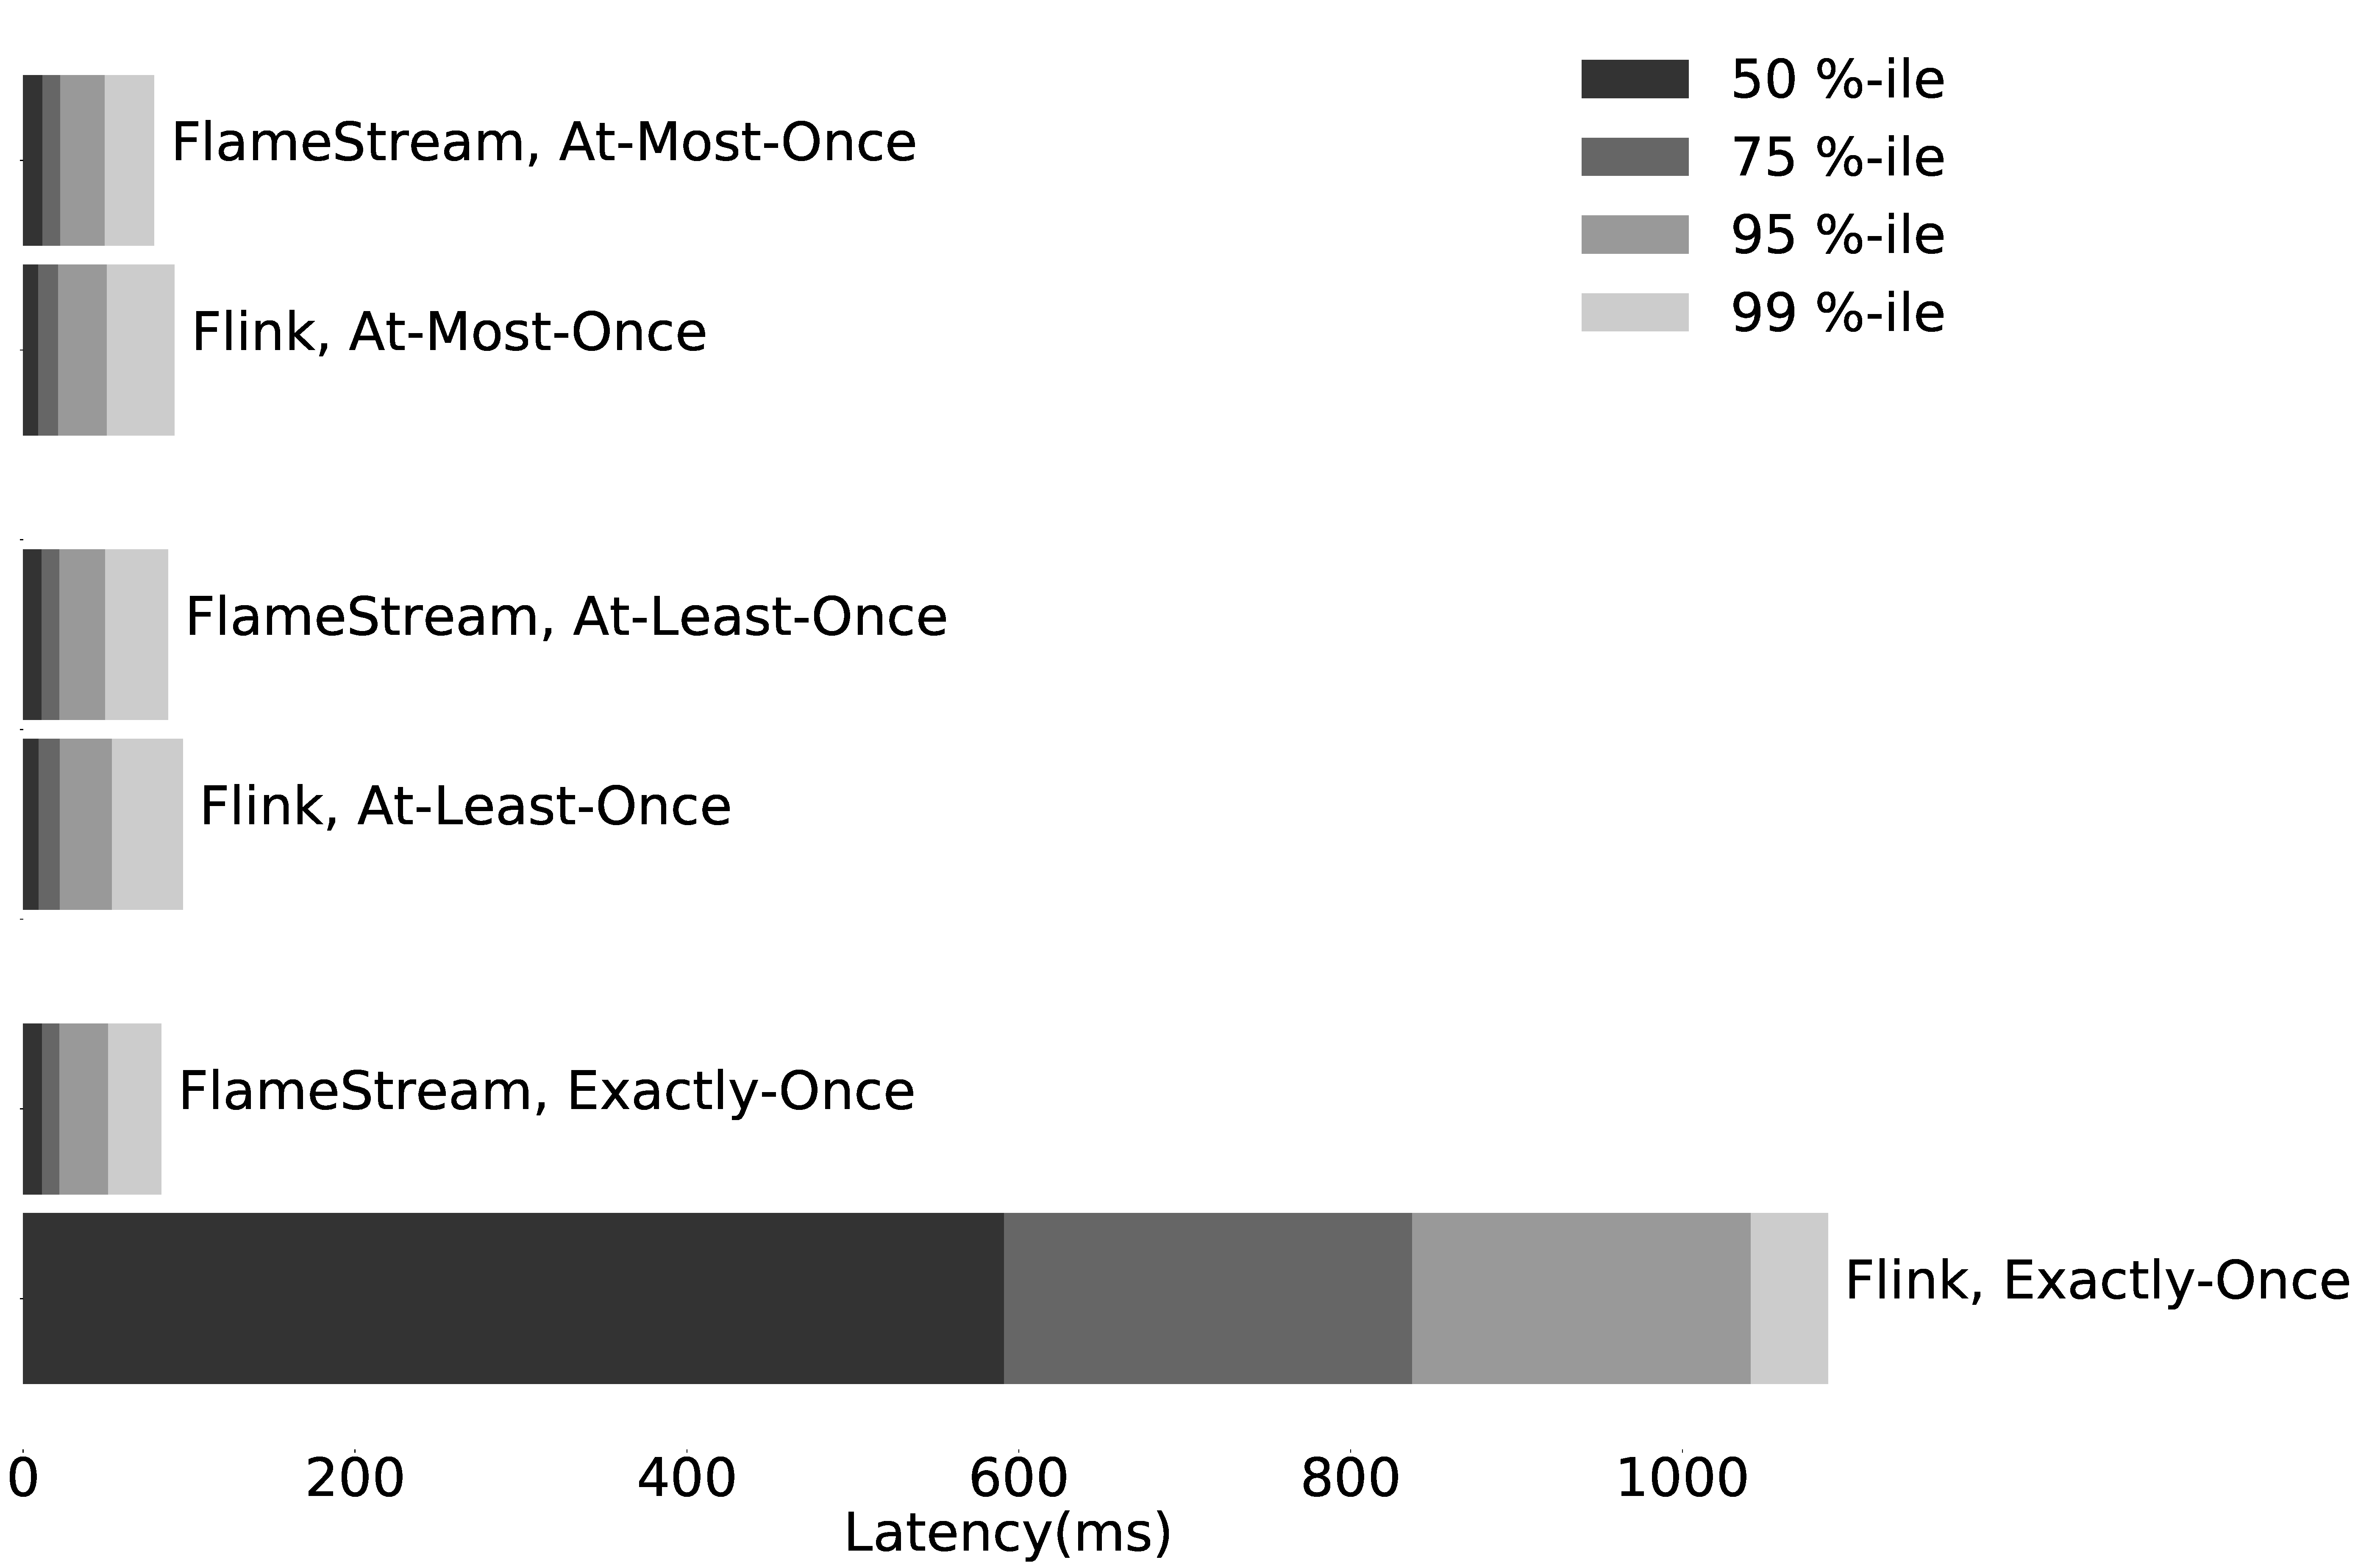
\includegraphics[width=.5\textwidth]{pics/comparison1000}
  \caption{The comparison in latencies between \FlameStream\ and Flink with 1000 ms delay between checkpoints}
  \label {comparison1000}
\end{figure}
